\documentclass[a4paper, 12pt]{article} % Font size (can be 10pt, 11pt or 12pt) and paper size (remove a4paper for US letter paper)

\usepackage[protrusion=true,expansion=true]{microtype} % Better typography
\usepackage{graphicx} % Required for including pictures
\usepackage{wrapfig} % Allows in-line images
\usepackage{german}
\usepackage{ngerman}
\usepackage{url}

\usepackage{mathpazo} % Use the Palatino font
\usepackage[T1]{fontenc} % Required for accented characters
\linespread{1.05} % Change line spacing here, Palatino benefits from a slight increase by default

\makeatletter
\renewcommand\@biblabel[1]{\textbf{#1.}} % Change the square brackets for each bibliography item from '[1]' to '1.'
\renewcommand{\@listI}{\itemsep=0pt} % Reduce the space between items in the itemize and enumerate environments and the bibliography

\renewcommand{\maketitle}{ % Customize the title - do not edit title and author name here, see the TITLE block below
\begin{flushright} % Right align
{\LARGE\@title} % Increase the font size of the title

\vspace{50pt} % Some vertical space between the title and author name

{\large\@author} % Author name
\\ \vspace{10pt}\@date % Date

\vspace{40pt} % Some vertical space between the author block and abstract
\end{flushright}
}

%----------------------------------------------------------------------------------------
%	TITLE
%----------------------------------------------------------------------------------------

\title{\textbf{VU IT-Strategie �bung 1}\\ % Title
WS 2013\\\vspace{5pt}
Gruppe 03} % Subtitle

 

 

 
\author{Hafellner Markus (1125415)\\
 Lin Zhong Li (0828454)\\
 Prybila Christoph (0925463)\\
 St�tz Anton (1129424)\\
 \vspace{10pt}
 \textbf{Gew�hlte Branche:} Banken
\\{\textit{Innovationsfelder: mobile banking, big data, contactless payment}}} % Institution

%----------------------------------------------------------------------------------------

\begin{document}

\maketitle % Print the title section

\newpage

\tableofcontents

\newpage

%----------------------------------------------------------------------------------------
%	ESSAY BODY
%----------------------------------------------------------------------------------------

\section{Kontextbezogene Recherchen}
\subsection{IT-Strategie im digitalen Zeitalter allgemein}
\label{subsec:StrategieAllgemein}

%%%%%%%%%%%%%%%%%%%%%%%%%%%%%%%%%%%%%
\subsubsection{IT-Strategie im Kontext der ``Digitalen Transformation'' moderner Unternehmen}

\glqq An effective IT strategy that forms an integral part of the
business strategy is imperative ...\grqq

In einer durchgef�hrten Studie wurde gezeigt, dass es zwar den Versuch gibt eine IT-Strategie zu formulieren, jedoch stellt sich in der Praxis meistens heraus, dass diese nicht sehr effektiv ist. Mehrere Gr�nde werden daf�r sind: keine Koppelung mit business processes, keine Koppelung mit der Unternehmensstrategie, die organisatorischen Bereiche des Unternehmens wurden nicht richtig eingebunden und es gab eine ineffektive Koordinierungsstelle. Des Weiteren wurde gezeigt, dass sich die IT-Strategie zwar mit den technischen Aspekten befasst, jedoch zu wenig mit den organisatorischen Aspekten.
\cite{808363}
\\

Die zwei gr��ten H�rden in Unternehmen heutzutage sind, dass Verstehen des Wertes der IT und die richtige Ausrichtung der IT im Unternehmen. Oft kommt es auch vor, dass die IT-Strategie sehr Technik lastig ist, und es f�r Gesch�ftspartner schwer ist diese zu verstehen.
\cite{4339647}
\\

Die Umwelt von Unternehmen ver�ndert sich stetig mit der Weiterentwicklung bestehender und neuer Technologien. Hierf�r ist es wichtig, dass Unternehmen ihre Gesch�ftsprozesse anpassen und entsprechend ver�ndern. Demnach muss man darauf achten, dass Unternehmen m�glichst flexible Management-Informationssysteme besitzen, um immer die aktuellen Modelle des Managements abbilden zu k�nnen. Eine IT-Strategie hat den Zweck Informationssystem zu verbessern und bessere Dienste f�r die Management-Strategie zu leisten.
\cite{5304653}
\\

In den letzten Jahren ist eine interessante Transformation bei IT-Systemen zu beobachten. Es werden von vielen gro�en und Namhaften IT-Unternehmen Dienste �ber das Internet(eine sogenannter Web-Service) angeboten, die von Unternehmen gekauft werden k�nnen. Dies f�hrt die Unternehmen weg davon all ihre Hardware und Software selbst zu verwalten. Des Weiteren erf�hrt das Unternehmen durch diese neue Strategie einen immensen Kostenvorteil.
\cite{Strategy_Harvard}
\\

Unternehmen in allen Sektoren werden immer abh�ngiger von einer Informations- und Kommunikationstechnolgie, aufgrund einer immer und stetig weiterentwickelnden IKT-Technologie. Dennoch werden die Gesch�ftserwartungen der IT oft nicht eingehalten, da es Probleme bei der Durchf�hrung der IT-Strategie und schlechte Kontrollmechanismen gibt.
\cite{Velitchkov:2008:ISE:1500879.1500955}
%%%%%%%%%%%%%%%%%%%%%%%%%%%%%%%%%%%%%

%%%%%%%%%%%%%%%%%%%%%%%%%%%%%%%%%%%%%
\subsubsection{Auswirkungen von Smart Technologies, Social Apps etc. auf unternehmensinterne Prozesse}
Durch ihr rasantes Wachstum und gesellschaftliche Durchdringung, werden Soziale Medien immer st"arker Teil von unternehmensinternen Prozessen. Die Relevanz von Sozialen Applikationen und Technologien ist jedoch von Unternehmen zu Unternehmen unterschiedlich und schwierig zu messen. Dies macht es oftmals schwer zu entscheiden den Trend zu folgen oder auszulassen.
\cite{Nair2011}

Allgemein jedoch, k"onnen Unternehmen Soziale Medien, mittels Analysewerkzeugen, als Verhaltens- oder Kompetenzdatenbanken ihrer eigenen Mitarbeiter verwenden. Durch die Analyse von Meinungen und Verhaltensmustern von Mitarbeitern k"onnen versteckte arbeitstechnische Aspekte und informelle Abl"aufe innerhalb des Unternehmens beleuchtet werden. Solche Informationen k"onnen dann in weitere Folge im internen Human-Ressource (HR) Management oder bei der Definition von Business-Prozessen verwendet werden. \cite{Sinha2012}

Das voranschreiten von Cloud-Technologien erm"oglicht die Entwicklung von internen Abl"aufen in eine andere Richtung. Die Cloud erm"oglicht das Auslagern von It-Infrastruktur und anderen Aktivit"aten um diese nur noch als ''Service'' in das Unternehmen einzubinden. Dynamische Skalierung um Spitzenlasten abzufangen ist ein weiterer Vorteil dazu. Diese Tendenz zum Auslagern kann auch auf ganze Business-Prozesse oder das Business-Prozess-Management angewendet werden. Mittels ''Business-Process- as - a - Service'' (BPaaS) k"onnen interne Prozesse teilweise oder sogar komplett ausgelagert werden. \cite{Stoitsev2012}

Bei einem hohen Grad an Automatisierung k"onnen Business-Prozesse teilweise komplett in die Cloud ausgelagert werden. Durch dynamisches Skalieren und Business-Prozess "as-a-service" Clouds k"onnen Kunden eigens zugeschnittene Prozesse angeboten werden, welche dann in der Cloud durchgef"uhrt werden. Dieser Ansatz muss jedoch mit klaren Kontrollmechanismen und Audits kombiniert werden um die Akzeptanz im Unternehmen zu gew"ahrleisten. Die exakte Kontrollierbarkeit der Prozesse zu gew"ahrleisten ist in diesem Fall die gr"o"ste Herausforderung. \cite{Accorsi2011}
%%%%%%%%%%%%%%%%%%%%%%%%%%%%%%%%%%%%%

%%%%%%%%%%%%%%%%%%%%%%%%%%%%%%%%%%%%%
\subsubsection{Auswirkungen von Smart Technologies, Social Apps etc. auf Kunden und externe Prozesse}
Der Mittelpunkt von Smarten Technologien und Sozialen Medien ist die Interaktion von deren Nutzern. Diese Technologien und Medien erleben seit Jahren ein rasantes Wachstum. In seinen Anf�ngen brauchte das Internet nur vier Jahre um 50 Millionen Nutzer zu erreichen. Facebook wuchs um 50 Millionen Nutzer in nur einem halben Jahr. \cite{Nair2011} Nutzerinteraktion bezieht sich dabei einerseits auf den Konsum von Inhalten, aber auch das Erstellen von Inhalten selbst. \cite{Alt2012}

Durch die Abwanderung zu neuen digitalen Medien verlieren die urspr�nglichen Printmedien, Radio oder Fernsehen zunehmend an Bedeutung. Echtzeit-Information wird ein integrales Element f�r Kundenverhalten. \cite{Hennig2010}

Durch diese fortschreitende Verbreitung von mobilen Technologien, wird Kommunikation auch zusehends Orts- und Situationsabh�ngig. \cite{Alt2012} Diese neuen M�glichkeiten der Interaktion ver�ndert auch das verhalten von Kunden. Dies gilt vor allem f�r die Art und Weise wie Information �ber Unternehmen und Produkte gesammelt und ausgetauscht werden. \cite{Hennig2010} Smarte Technologien und Soziale Applikationen geben Konsumenten die verschiedensten M�glichkeiten aktiv Informationen �ber Produkte und Dienste anzubieten. \cite{Foster2010} Durch Plattformen wie Ebay oder Amazon werden Konsumenten auch zu Verk�ufern ihrer eigenen Produkte.

Unternehmen m�ssen sich durch dieses ver�nderte Kommunikationsverhalten auf neue  Herausforderung im Bereich des Customer-Relationship-Managements (CRM) einstellen. Der mittelbare Kundenkontakt ver�ndert sich. Auߟendienstmitarbeiter, Kundenberater oder Call-Center-Agenten verlieren an Bedeutung. Kunden erwarten einen unmittelbaren mit den Unternehmen. \cite{Alt2012} Sie werden zu aktiven und stark vernetzten Partnern, welche auch die Rolle von Anbietern und Produzenten einnehmen k�nnen. Dies macht es f�r Unternehmen schwieriger das eigene Marken-Image und das Klima von Kundenbeziehungen zu kontrollieren \cite{Hennig2010}

Es ergeben sich viele neue Risiken f�r Unternehmen im Umgang mit sozialen Medien. Kunden geben den Erfahrungen und Meinungen anderer Konsumente h�heren Stellenwert und Glaubw�rdigkeit gegen�ber der Unternehmenskommunikation. Eskalierte Diskussionen in sozialen Medien k�nnen starke negativen Auswirkungen auf Unternehmen haben diese sp�t oder gar nicht daran teilnehmen. \cite{Alt2012}

Gleichzeitig gibt es auch viel Potential f�r neue Kommunikationsformen zwischen Kunden und Unternehmen. Unternehmen bekommen die M�glichkeit direkt mit ihren Kunden zu interagieren um sich �ber Kampagnen oder Probleme auszutauschen. Oftmals wird eine solche direkte Interaktion von den Kunden auch erwartet. \cite{Alt2012}

Besonders f�r Unternehmen mit Endkundenkontakt ist die Nutzung des SocialWeb eine wettbewerblichen Notwendigkeit. Gleichzeitig darf der Einsatz von neuen Medien, �ltere Konsumenten nicht ausschlie�en. Der Kontakt zu Konsumenten aus �lteren Bev�lkerungsschichten darf nicht vernachl�ssigt werden. \cite{Coughlin2007}
%%%%%%%%%%%%%%%%%%%%%%%%%%%%%%%%%%%%%

%%%%%%%%%%%%%%%%%%%%%%%%%%%%%%%%%%%%%
\subsubsection{Erkenntnisse der grossen Industrieanalysten}
Im heutigen digitalen Zeitalter ist es auch zunehmend wichtiger geworden die Erkenntnise von gro"sen Industrieanalysten f"ur die Strategie im Bereich der Informationstechnologien eines modernen Unternehmens in Betracht zu ziehen. Zu den heutigen gro"sen Marktf"uhren dieser Branche z"ahlen Firmen wie Forrester Research Inc., Gartner Inc., IDC Corporate oder auch Frost \& Sullivan. Jeder der genannten Firmen besch"aftigt mehr als 1000 Analysten, die weltweit f"ur ihre Kunden Trends erforschen, den globalen Markt analysieren sowie Prognosen f"ur die Zukunft erstellen. Deren Forschungen und Analysen sollen dabei in Hinblick auf die IT Strategie eines modernen Unternehmen als Entscheidungsunterst"utzung dienen um in der rapide wachsenden und kontinuerlich wandelnden IT Branche wettbewerbsf"ahig zu bleiben sowie f"ur die zuk"unftigen Herausforderungen optimal ger"ustet zu sein. 

Bevor begonnen wird ein Konzept f"ur eine IT Strategie zu erstellen bzw. sp"ater Schritt f"ur Schritt umzusetzen, m"ussen zuerst die Werte, Visionen und Ziele eines Unternehmens auskommuniziert und verinnerlicht werden. Jede technologische Strategie beruht auf der Unternehmensstragie, daher ist es in dieser Hinsicht besonders von Vorteil, diese beiden Vorgehen auf einander abzustimmen um Komplikationen, die insbesondere das Erreichen der Ziele erschweren, zu vermeiden.
 
Forrester Research Inc. bezeichnet die Wechselwirkung von Technologie und Gesch"aftsstrategie als Business Technology Strategy. Im heutigen digitalen Zeitalter ist die Effizienz einer Unternehmensstrategie stark abh"angig von der technologischen Komponente. Firmen k"onnen nur l"angerfristig erfolgreich sein und ihr volles Potenzial aussch"opfen, wenn sie die n"otigen Kompetenzen besitzen, technologische Ressourcen und Innovationen komplett in ihre Gesch"aftsstrategie zu integrieren. \glqq Business Technology Strategy must start with business and end with business. \grqq  

Der traditionelle Ansatz des Wasserfallmodells zur Entwicklung einer Strategie eines Unternehmen gilt schon lange als general"uberholt und w"urde den Herausforderungen und Anforderungen der heutigen Zeit nicht gewachsen sein. Stattdessen sollen die Entscheidungstr"ager eines Unternehmens einen agilen und iterativen Ansatz verfolgen. Die Marktverh"altnisse "andern sich "au"serst h"aufig und sehr rasant, umso wichtiger ist es hier schnell auf die Ver"anderungen zu reagieren und die Strategie entsprechend der neuen Anforderungen zu adaptieren\cite{ForresterResearch}. 
%%%%%%%%%%%%%%%%%%%%%%%%%%%%%%%%%%%%%

%%%%%%%%%%%%%%%%%%%%%%%%%%%%%%%%%%%%%
\subsubsection{Erkenntnisse der grossen Beratungsunternehmen}
"Ahnlich wie bei den Erkenntnisen der Industrieanalysten spielt auch die Meinung der gro"sen Consultingunternehmen eine wichtige Rolle in Bezug auf gut konzipierte IT-Strategien. Zu den weltweit umsatzst"arksten Anbieter in dieser Branche z"ahlen McKinsey \& Company Corporation, Accenture PLC., Deloitte Consulting und Capgemini S.A, wobei j"ahrlich Ums"atze in Milliardenbereich erzielt werden. In erster Linie ist deren Kerngesch"aft ihre Beratung als Dienstleistung anderen Unternehmen anzubieten. Sie beraten das Management oder Entscheidungstr"ager in allen m"oglichen Branchen beim Prozess der Entscheidungsfindung.

Vor allem im Bereich IT Business sind sehr viele Beratungsunternehmen fokussiert. Nicht zuletzt aufgrund der immer st"arker wachsenden und st"andig im Wandel befindlichen technologischen Herausforderungen, sind viele Firmen gezwungen, sich an die Kompetenzen, Wissen und Erfahrungen von Consultern zu st"utzen. Im heutigen digitalen Zeitalter bedarf es moderner und innovativer IT Strategien um nachhaltig die Kosten zu senken, Produktivit"at zu steigern, Gesch"aftseffizienz und -effektivit"at zu verbessern sowie letztendlich sich erfolgreich am Markt zu etablieren. Der Einsatz von technologischen Komponenten im Einklang mit der Unternehmensphilosophie verschafft einen gro"sen Vorteil und durch dieses Zusammenwirken ist man in der Lage die Ziele des Unternehmens schneller zu erreichen. 

Laut Accenture werden im digitalen Zeitalter Business und IT Strategie zusammen verschmelzen, so dass eine klare Abgrenzung nicht mehr m"oglich ist. Jeder Gesch"aftsprozess ohne technologischen Einfluss wird in Zukunft kaum vorstellbar sein. Neue, innovative Technologien wie beispielsweise das Cloud Computing, das stetig an Popularit"at gewinnt und des "ofteren auch schon in vielen Gesch"aftsbereichen Einsatz findet, werden in naher Zukunft die Strategien vieler Unternehmen beeinflussen und pr"agen.\cite{AccentureConsulting}
%%%%%%%%%%%%%%%%%%%%%%%%%%%%%%%%%%%%%

%%%%%%%%%%%%%%%%%%%%%%%%%%%%%%%%%%%%%
\subsubsection{Erkenntnisse der grossen ICT-Unternehmen}
Um eine eigene IT Strategie zu entwickeln ist es oft sinnvoll, sich an Modellen die schon in der Praxis angewendet werden und funktionieren ein Beispiel zu nehmen. So ist es nicht verwunderlich, dass gro"se ICT Unternehmen wie IBM, Atos, Microsoft, Google und Apple - um nur ein paar zu nennen - darauf einen gro"sen Einfluss nehmen. Diese Unternehmen sind federf"uhrend in der Entwicklung, Implementierung und Bereitstellung von neuen IT Strategien wie Cloud Services, SOA und "Ahnlichem.\\

In den letzten Jahren zeigt sich ein Trend der immer weiter richtung Cloud Computing und Software as a Service (SaaS) geht. Die Vorteile liegen auf der Hand: (1) Die Illusion von endlos zur Verf"ugung stehenden Ressourcen, (2) das Fehlen von Verpflichtungen bevor man die Cloud benutzt und (3) die M"oglichkeit f"ur ben"otigte Ressourcen (Speicher, Rechenleistung, usw.) nur bei Gebrauch zu bezahlen. Diese Flexibilit"at ist vor allem f"ur kleine Unternehmen und Start-Up Unternehmen von enormem Vorteil ~\cite{Armbrust2009}. Dadurch ist es auch nicht verwunderlich, dass die Vorreiter in Punkto IT-Strategie Atos, Microsoft und Google mit Canopy, Microsoft Azure und Google Appengine bereits jeweils ein Cloudservice f"ur die public und auch private Cloud anbieten.\\

Bei der Wahl der richtigen IT-Strategie geht es laut IBM und Atos haupts"achlich um (1) die Bereitschaft der CxOs, (2) die bessere Vereinigung von IT Ressourcen, Investitionen und Gesch"aftsstrategien, (3) eine erh"ohte Effektivit"at und Effizienz des Einsatzes von IT Ressourcen und verminderte Betriebskosten, (4) die Wahl einer richtigen Cloud Strategie, (5) die Wahl einer richtigen Green IT Strategie, (6) effizienterer Einsatz von vorhandenen Ressourcen, (7) h"oherer Nutzen von Sicherheitsma"snahmen, (8) die Einhaltung von beh"ordlichen Regeln und Bestimmungen.


%%%%%%%%%%%%%%%%%%%%%%%%%%%%%%%%%%%%%


\subsection{Herausforderungen und Strategien f�r die Branche ``Banken''}

%%%%%%%%%%%%%%%%%%%%%%%%%%%%%%%%%%%%%
\subsubsection{Aktuelle Herausforderungen und Trends in der gew�hlten Branche}
\glqq The financial services industry has been transformed substantially over the last decade.\grqq
\cite{1508397} 
\\

Die immer gr��er werdende Vorherrschaft von Smartphones und dem Internet, ist eine gute Grundlage f�r das Wachstum von mobile banking. Normalerweise verwendet man mobile banking f�r das Anzeigen des aktuellen Saldos des Kontos oder f�r �berweisungen, jedoch kann man kein Bargeld beheben. Der Vorteil von mobile banking ist die Kostenersparnis f�r die Banken, da der Kunde ohne zu tun von Bankangestellten oder des Besuchs einer Bankfiliale viele Bankgesch�fte erledigen kann. Au�erdem erh�ht es den Umsatz von Anbietern mobiler Dienste, da man f�r die Nutzung mobiler Dienste Geld verlangen kann. Ein weiterer Vorteil von mobile banking ist die M�glichkeit der Erschlie�ung neuer M�rkte, bei der �rmeren Bev�lkerung.
\cite{5723885}
\\

Die immer weiter wachsende Bev�lkerung von  China bietet gro�e Herausforderungen und Chancen f�r den Bankensektor. Insgesamt gab es 2007 210 Millionen Internetuser, davon nutzten 19,2\% internet banking. Wichtig hierbei ist, dass man dem Kunden vermittelt, wie einfach internet banking zu benutzen ist.
\cite{4680308}
\\

Die rasche Entwicklung von mobile-commerce Applikationen, wie mobile banking revolutionieren den Bankensektor. Mobile banking erlaubt den Zugriff auf die Bankdienste zu jeder Zeit und an jedem Ort. Jedoch sind die mobilen Endger�te anf�llig f�r Angriffe durch Dritte, deshalb ist die Sicherheit ein wesentliches Thema in diesem Bereich. Es ist wichtig geeignete kryptografische Verfahren beim Transfer der Daten einzusetzen, um die Daten der Kunden zu sch�tzen.
\cite{4812913}
\\

Besonders in Schwellenl�ndern k�nnte mobile banking zum prim�ren Kanal zwischen Bank und Kunde werden. Es wird auch erwartet, dass m-banking das Kreditkartensystem und das klassische netbanking ersetzen wird. Auch der Druck auf der Kundenseite wird in den n�chsten Jahren zunehmen, da es immer billigere Endger�te am Markt gibt, die f�hig sind mobile-banking zu unterst�tzen.
\cite{5169360}
\\

Eine gro�e Herausforderung in Schwellenl�ndern ist jedoch beim mobile banking die gr��ere Verbreitung, da es unterentwickelte Telekommunikationseinrichtungen und eine geringe Bekanntheit von m-banking gibt. 
\cite{5286659}


%%%%%%%%%%%%%%%%%%%%%%%%%%%%%%%%%%%%%

%%%%%%%%%%%%%%%%%%%%%%%%%%%%%%%%%%%%%
\subsubsection{Darstellung der wesentlichen technologischen Treiber}
Die heutige Generation lebt immer mehr vom Trend der Smartphones und Tablets. \glqq Jeder Mensch\grqq in den westlichen Staaten besitzt ein Smartphone, viele mitunter auch noch ein Tablet und zu guter Letzt auch noch ein Notebook und/oder einen Stand-PC. Diese Menge an Ger�ten mit denen Informationen aus dem Internet konsumiert werden k�nnen, stellt ganz neue Herausforderungen an angebotene Dienste von Unternehmen. So ist es heutzutage ein Muss, dass die Funktionen, die auf der Desktopoberfl�che zur Verf�gung stehen auch am Tablet oder Smartphone benutzbar sind. Jedoch in einer Darstellung die an die neuen Hardwarebedingungen angepasst ist. Ein Kunde m�chte somit in der Bank und auf jedem seiner Ger�te die gleichen Funktionen wie In- und Auslands�berweisung, Kontoauszug, das Sperren etwaiger Karten und vieles Mehr zur Verf�gung haben. Diese Vielfalt von Funktionen zu jeder Zeit an jedem Ort wird als \textit{Multi-Channel Banking} bezeichnet und ist zurzeit eines der wichtigsten Themen in der Bankenbranche. ~\cite{Cortinas2010}\\

Der Begriff \textit{Self-Service Technology} ist sehr verwandt mit dem \textit{Multi-Channel Banking}. Es geht dabei darum, dem Benutzer die M�glichkeit zu bieten, die Dienste die auf herk�mmliche Weise bei einem Bediensteten der Bank in Auftrag gegeben wurden und daraufhin erledigt wurden, nun selbst zu erf�llen. Diese neue Art der \glqq Bedienung\grqq wird vor Allem dadurch m�glich, dass die Verbreitung des Internets und die Zugriffsm�glichkeiten darauf durch mobile Endger�te stetig ansteigt. Diese neue \textit{Self-Service Technology} bietet dar�ber hinaus nicht nur dem Kunden Vorteile, da er von Ort und Zeit ungebunden die gew�nschten Bankgesch�fte durchf�hren kann, sondern ist auch als Strategie f�r Unternehmen �u"serst interessant, da das Personal mit direktem Kundenkontakt dadurch reduziert werden kann, als doch der Kunde pers�nlich diese Aufgaben erledigt.
Bei all den positiven Seiten darf jedoch nicht darauf vergessen werden, dass der erfolgreiche Einsatz von \textit{Self-Service Technology} und die dazugeh�rige Akzeptanz beim Kunden nur realisierbar ist, wenn bei eingesetztem \textit{Multi-Channel Banking} die angebotenen Services in jedem Channel nutzbar sind. ~\cite{Eriksson2007} \\

Um Geldtransaktionen zwischen unterschiedlichen Partnern im Internet einfacher machen zu k�nnen wurden sogenannte \textit{Web ATMs} entwickelt. Dabei handelt es sich um ein Verfahren, das dem eines EC-Karten Terminals nachgeahmt wurde. Das Bezahlen von zum Beispiel Hotelrechnungen im Internet war immer mit gewissen M�hen verbunden. So bekam man nach der Onlinebuchung zuerst eine Reservierungsbest�tigung mit Vorbehalt. Danach musste man eine �berweisung an das Hotel t�tigen und eine �berweisungsbest�tigung an den Transaktionspartner schicken. Da es sich im Unternehmen wiederum um unterschiedliche Abteilungen zur Bearbeitung von Rechnungen/Einzahlungen und Buchungsbest�tigungen handelte, konnte bis zur endg�ltigen Zusage eines Zimmerplatzes einiges an Zeit vergehen. Durch \textit{Web ATMs} ist es nun m�glich, sofort nach der Buchung auf eine Seite der Bank weitergeleitet zu werden, wo man durch Angabe der Kontodaten die �berweisung t�tigen kann und sowohl der Kunde als auch das Unternehmen sofortige Gewissheit �ber den Erfolg der Transaktion erhalten. Somit kann auch die fixe Zusage eines Zimmers gleich nach R�ckkehr auf die Unternehmensseite erfolgen. ~\cite{Tsai2010}


%%%%%%%%%%%%%%%%%%%%%%%%%%%%%%%%%%%%%

%%%%%%%%%%%%%%%%%%%%%%%%%%%%%%%%%%%%%
\subsubsection{Strategieempfehlungen der Experten}
Lange Zeit war es gang und g�be im Bankensektor auf aufwendige Eigenl�sungen zur�ckzugreifen. Mit den immer steigenden Anforderungen an Banken im europ�ischen Raum, zusammen mit immer strikter werdenden gesetzlichen Regelungen, ist es f�r Banken zunehmend schwieriger auf all diese �nderungen in angemessener Zeit und mithilfe der gegebenen Ressourcen zu reagieren. F�r die meisten Banken ist die Verwendung und st�ndige Anpassung einer (teils) komplett veralteten Eigenl�sung nicht mehr leistbar, auch weil das ben�tigte Know-How in Form von Mitarbeitern zunehmend am Ende der Lebensarbeitszeit ist. Dadurch werden moderne Standardsoftware und Outsourcingstrategien immer interessanter.~\cite{Berger2012}\\
Auch bei den Sourcingstrategien vollzieht sich seit den letzten Jahren ein Wandel in Richtung \textit{Multiple-Sourcing}. Dies war im Finanzdienstleistungssektor lange ein Tabuthema, da die Integrationskosten f�r zu hoch erachtet wurden und den entstehenden Effekt der erh�hten Ausfallsicherheit zu rechtfertigen. Doch mit dem derzeitigen Stand der IT-Technik und der zunehmenden Verbreitung von Standards durch den Einsatz von Standardsoftware ist es laut Buhl ~\cite{Buhl2011} auch in der Finanzdienstleisterbranche denkbar und von Vorteil eine \textit{Multiple-Sourcing} Strategie einzusetzen.
%%%%%%%%%%%%%%%%%%%%%%%%%%%%%%%%%%%%%

%%%%%%%%%%%%%%%%%%%%%%%%%%%%%%%%%%%%%
\subsubsection{Themenf�hrer, Meinungsmacher und Think Tanks in der gew�hlten Branche}

Eines der wichtigsten Themen im Bankensektor ist die Sicherheit der IT-Infrastruktur. Aus diesem Grund wurden in einigen Industrienationen eigene Abteilungen eingerichtet, welche die Risiken von IT-Systemen �berwachen. Wie zum Beispiel die American Monetary Administration oder die Hong Kong Monetary Authority. Amerika spielt in diesem Bereich eine besondere Vorreiterrolle, waren sie doch das erste Land welches ein IT-Risikomanagement eingerichtet haben.
\cite{5592630}
\\

Ein Problem bei IT basierten Bank-Applikationen im allgemeinen ist die Authentifizierung des Kunden. Da es durch Hackerangriffe passieren kann, dass Passw�rter gestohlen werden, wird von einer Expertengruppe vorgeschlagen das Passwort des Kunden mit einem verbesserten Steganographie-Verfahren zu verstecken. Dieser verbesserte Algorithmus verwendet mehr Zielpixel, sodass die Unwahrnehmbarkeit steigt. Darauf folgend werden die Zielpixel aufgeteilt zwischen der Bank und dem Kunden, um das Passwort nun rekonstruieren zu k�nnen ben�tigt man beide Teile. Zudem hat dieses Verfahren den Vorteil, dass man mit einer Kompromittierung der Bank oder des Kunden nicht das Passwort rekonstruieren kann.
\cite{6203923}
\\

Besonders die Entwicklung von Software die im Finanz- und Bankenbereich eingesetzt wird muss speziellen Qualit�tsanforderungen gen�gen, da diese sicherheitskritische Software in einem Fehlerfall zu einem signifikanten Verm�gensverlust f�hren kann.
\cite{6407380}
\\

Eine Vorreiterrolle in Sachen mobile-payment sind Schwellenl�nder. Tom Standage, hat in einem Artikel des Economist gesagt, dass es einfacher ist mit einem Mobiltelefon in Nairobi zu bezahlen, als in New York. Kenia hat mit Stand Februar 2012 18 Millionen mobile-payment Kunden. Generell wird f�r den Asien-Pazifik Raum ein gro"ses Wachstum vorhergesagt.
\cite{6248655}
\\

In China ist der Bankensektor gerade im Wandel, die gr�"sten Banken Chinas bewegen sich weg von den weltweit gr�"sten Privatkundenbanken hin zu gut integrierten Finanzdienstleistern mit hochverf�gbaren Bank-Applikationen und big data business. Jedoch sind die momentan genutzten Rechenzentren der Banken nicht daf�r ger�stet. Eines der schwierigsten Ziele ist das Ausrollen des Next Generation Banking Systems. Dies ist die gr�"ste Umstellung f�r Banken mit �ber 5000 physikalischen Servern und noch mehr virtualisierte Ressourcen in einer privaten Cloud. Eine der gr�"sten Banken, die an dieser Umstellung beteiligt sind ist, die China Industrial and Commercial Bank of China Limited(ICBC) besitzt insgesamt 282 Millionen Kunden.
\cite{6649734}


%%%%%%%%%%%%%%%%%%%%%%%%%%%%%%%%%%%%%

%%%%%%%%%%%%%%%%%%%%%%%%%%%%%%%%%%%%%
\subsubsection{Statistiken, Visualisierungen und Konzeptdarstellungen}
Mit zunehmend signifikanteren Fortschritten im Bereich der Informationstechnologien sind mobile Endger"ate wie Smartphones oder Tablets kaum mehr aus dem Alltag wegzudenken. Mit der Zahl der mobile Devices steigt auch der Bedarf der mobilen Services. Vor allem in der Bankenbranche hat sich in den letzten Jahren der Trend des internet bzw. mobile Banking etabliert und ist in heutigem digitalen Zeitalter zu einem fixem Bestandteil sowohl f"ur Firmen als auch Konsumenten geworden. 

Nach dem Motto: \glqq Customers can use services in wherever they want by location free access and at whenever they want by time free access. \grqq Der Benutzer besitzt alle Freiheiten wo und wann er welche Bankgesch"afte erledigen m"ochte. Insbesondere in S"udkorea, das weltweit zu den f"uhrenden L"andern der wireless Internet Technologien z"ahlt, ist die Anzahl der mobile banking Benutzern drastisch gestiegen. Die Bank of Korea ver"offentlichte quartalsm"a"sig die Daten des nationalen Transaktionsvolumens von internet sowie mobile banking Aktivit"aten.\cite{Jung2011}

\begin{figure}[h!]
	\caption{Anzahl der mobile banking Kunden in S"udkorea 2003-2010}
	\centering
		\includegraphics[scale=1.2]{figures/Jung2011}
\end{figure}

In der Bankbranche ist ein weiteres Innovationsfeld, das eng mit mobile banking verkn"upft ist, das Konzept des contactless payment. Mit dem rasanten Anstieg an mobilen Benutzern ist auch die Nachfrage nach sicherer und bequemer Bezahlung mit Hilfe eines mobilen Ger"ats gestiegen. Der gro"se Wachstum des mobile banking Sektors bietet den unterschiedlichsten Branchen viele M"oglichkeiten von diesem aufstrebenden Markt zu profitieren, inbesondere Mobiltelefonhersteller, Banken und Service Provider. Fr"uher oder sp"ater soll ein einziges mobiles Ger"at die klassische Brieftasche ersetzen. Eine M"oglichkeit des contactless mobile payment basiert auf der Technologie der Near Field Communication (NFC). Viele Mobiltelefone haben heutzutage schon einen NFC Microchip eingebaut, der es erm"oglicht innerhalb von zehn Metern per Funktechnik mit anderen NFC-f"ahigen Ger"aten zu kommunizieren. Somit hat man schon die M"oglichkeit kleine Geldbetr"age "uber Funk zu transferieren um beispielsweise einen Fahrschein mit seinem Smartphone zu kaufen ohne Bargeld oder Bankomat-/Kreditkarte bei sich zu haben. Folgende Abbildung zeigt die Darstellung eines NFC-basierten mobile payment Konzeptes\cite{Kadambi2009}:

\begin{figure}[h!]
	\caption{NFC-basierte mobile payment System}
	\centering
	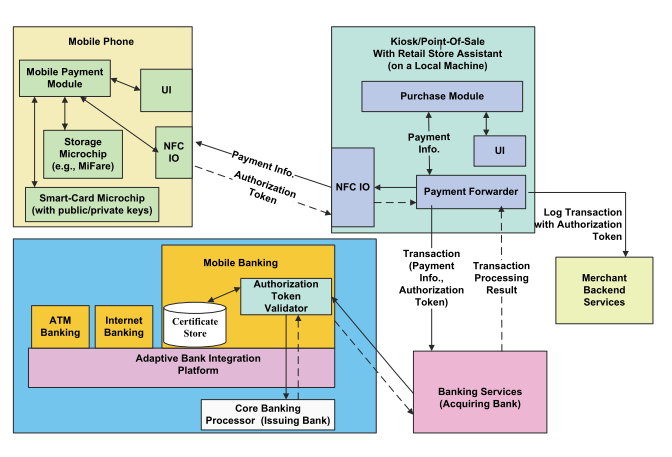
\includegraphics[scale=0.9]{figures/NFCmobilepayment}
\end{figure}
%%%%%%%%%%%%%%%%%%%%%%%%%%%%%%%%%%%%%

%%%%%%%%%%%%%%%%%%%%%%%%%%%%%%%%%%%%%
\subsubsection{Best Practices und interessante Fallbeispiele f�r branchenspezifische IT-Strategien}


Seit den 1970er-Jahren galt das Gesch�ftsmodell der Universalbank in den national abgeschotteten Bankenm�rkten der deutschsprachigen L�nder und in Frankreich als vorbildlich gegen�ber den Trennbankensystemen anglo-amerikanischer Pr�gung. Als bankbetriebswirtschaftliche Vorteile dieser Organisationsform von Banken wurde vor allem der horizontale Risikoausgleich zwischen den einzelnen Banksparten und die daraus resultierende geringere Krisenanf�lligkeit von Universalbanken gesehen. In Verfolgung der ?One-Bank-Strategie? entstanden Gro�banken, die durch ein umfassendes Angebot von Bankleistungen aus einer Hand in national abgegrenzten M�rkten ausreichend Werte schafften. Doch mit der Entwicklung zur Globalisierung der Bankm�rkte und zuletzt in der aktuellen Finanzmarktkrise zeigten sich Nachteile dieses traditionellen Branchen-Gesch�ftsmodells (Modell der integrierten Bank) hinsichtlich Wirtschaftlichkeit, Kundenkommunikation und Transparenz der Wertsch�pfung. Nachzugehen ist daher der Frage, wie neue Gesch�ftsmodelle mit schlanker Bankorganisationsform, auf Kundengruppen und Kundenbed�rfnisse fokussierten Angeboten spezialisierter Banken mit ?Multi-Bank-Strategie? den Anforderungen an hohe Wirtschaftlichkeit und an Generierung sowie Verteilung von Ertr�gen geeignet sein k�nnen, das Branchen-Gesch�ftsmodell nachhaltig weiterzuentwickeln. \cite{Bieger2011}
%%%%%%%%%%%%%%%%%%%%%%%%%%%%%%%%%%%%%

\bibliographystyle{unsrt}

\bibliography{references}

%----------------------------------------------------------------------------------------

\end{document}